%*****************************************
\chapter{Introduzione}\label{ch:introduction}

Negli ultimi anni molte branche della scienza e dell'industria si trovano a produrre e analizzare insiemi di dati sempre più grandi e complessi. Questi Big Data sono difficilmente analizzabili usando tecniche standard a causa di problemi sia tecnici che teorici.

Ad esempio, dover processare grandi quantità di dati complessi può avere facilmente un costo troppo elevato in termini di tempo e memoria rispetto alle possibilità della tecnologia odierna. Vi sono poi problemi che si annidano nell'analisi di dati in elevate dimensioni, in cui bisogna tenere conto di alcune particolarità, come il fatto che la distanza fra due punti smette di essere significativa.

Si può visualizzare questa cosa confrontando l'estrazione casuale di punti dal quadrato in dimensione 2 o dall'ipercubo in dimensione 100: estratti due punti $x$ e $y$ dalla distribuzione uniforme sull'ipercubo unitario in $\R^d$, la distanza fra loro è
\begin{equation*}
  d(x,y) = \sqrt{\sum_{i=1}^d (x_i - y_i)^2},
\end{equation*}
allora per la disuguaglianza di Hoeffding la distribuzione di $d(x,y)$ è concentrata attorno al valore medio per dimensioni $d$ elevate. In \cref{fig:pointdistance} si può vedere la differenza: i due grafici mostrano l'andamento della distanza di un punto casuale dell'ipercubo da altri 100 punti casuali per $d=2$ e $d=100$. Si può notare come all'aumentare della dimensione i valori si schiacciano attorno al valor medio.

\begin{figure}[ht]
  \begin{center}
    \begin{subfigure}[b]{.4\textwidth}
      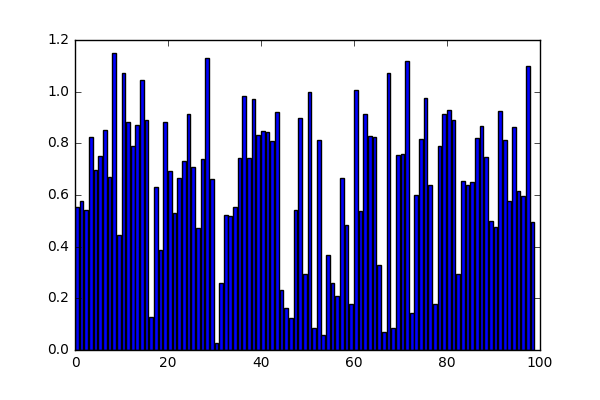
\includegraphics[width=\textwidth]{gfx/pltpoints2d.png}
      \caption{$d=2$}
    \end{subfigure}
    \begin{subfigure}[b]{.4\textwidth}
      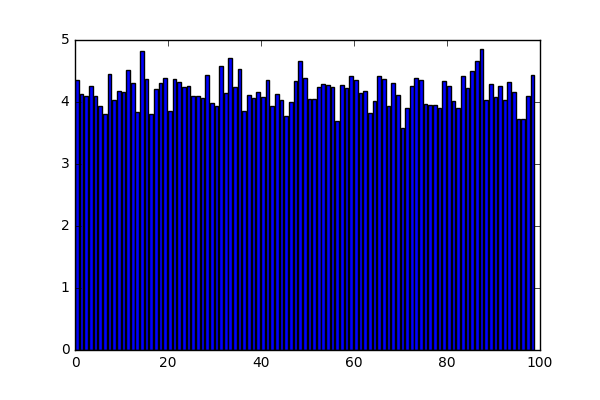
\includegraphics[width=\textwidth]{gfx/pltpoints100d.png}
      \caption{$d=100$}
    \end{subfigure}
    \caption{Distanza fra punti casuali nell'ipercubo}  \label{fig:pointdistance}
  \end{center}
\end{figure}

Ci interessa quindi sviluppare tecniche in grado di rivelare informazioni in spazi metrici di dimensione possibilmente elevata, in particolare vorremmo poter riassumere in un numero finito (piccolo) di variabili l'informazione che ci serve.

Utilizzeremo tecniche di topologia algebrica, e le informazioni che queste ci consentiranno di catturare riguardano la \emph{forma} dei dati. In dimensioni elevate è difficile visualizzare un insieme di punti e quindi comprendere se questo abbia una forma interessante, tuttavia utilizzando la topologia è possibile produrre una rappresentazione sintetica di uno spazio complesso mediante una quantità finita di informazioni, e tale che calcolando opportuni invarianti di questa rappresentazione si ricavino informazioni sulla \emph{forma} dello spazio. La topologia consente anche di esprimere mediante quantità precise cosa intendiamo per \emph{forma}.

Prendendo ad esempio la corona circolare in \cref{fig:annulus}, la proprietà che vogliamo essere in grado di catturare è il fatto che essa contiene essenzialmente un solo loop non banale a meno di omotopia, o in maniera equivalente potremmo dire che ha un unico foro.

\begin{figure}[ht]
  \begin{center}
    
\includegraphics[width=.5\textwidth]{gfx/annulus.pdf}
    \caption{Corona circolare}  \label{fig:annulus}
  \end{center}
\end{figure}

Vorremmo anche essere in grado di rappresentare sinteticamente uno spazio mediante simplessi, conservando quanta più informazione possibile sulla sua forma. Ad esempio passando dalla circonferenza al quadrato in \cref{fig:circsquare} perdiamo informazioni sulla curvatura, tuttavia le proprietà topologiche sono invariate.

\begin{figure}[ht]
  \begin{center}
    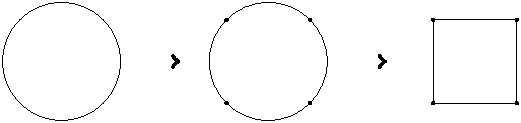
\includegraphics[width=.7\textwidth]{gfx/circsquare.pdf}
    \caption{Rappresentazione di una circonferenza}  \label{fig:circsquare}
  \end{center}
\end{figure}

Nel tipo di applicazione che ci interessa, tuttavia, l'oggetto di studio non è una varietà come nei casi precedenti, ma una nube di punti, cioé un sottinsieme finito di $\R^d$ o più in generale uno spazio metrico finito $X=\{x_1,\dots,x_n\}$. Anche in questo caso lo spazio può esibire una forma interessante, ad esempio in \cref{fig2:clusters} i dati si dispongono chiaramente in tre gruppi, mentre in \cref{fig2:circle} hanno chiaramente una forma circolare.

\begin{figure}[ht]
  \begin{center}
    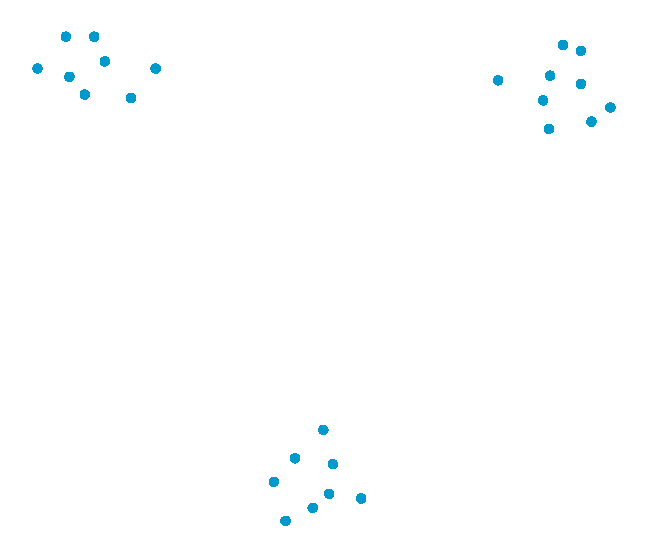
\includegraphics[width=.4\linewidth]{gfx/three_clusters_small.pdf}
    \caption{Dati divisi in più cluster}
    \label{fig2:clusters}
  \end{center}
\end{figure}

\begin{figure}[ht]
  \begin{center}
    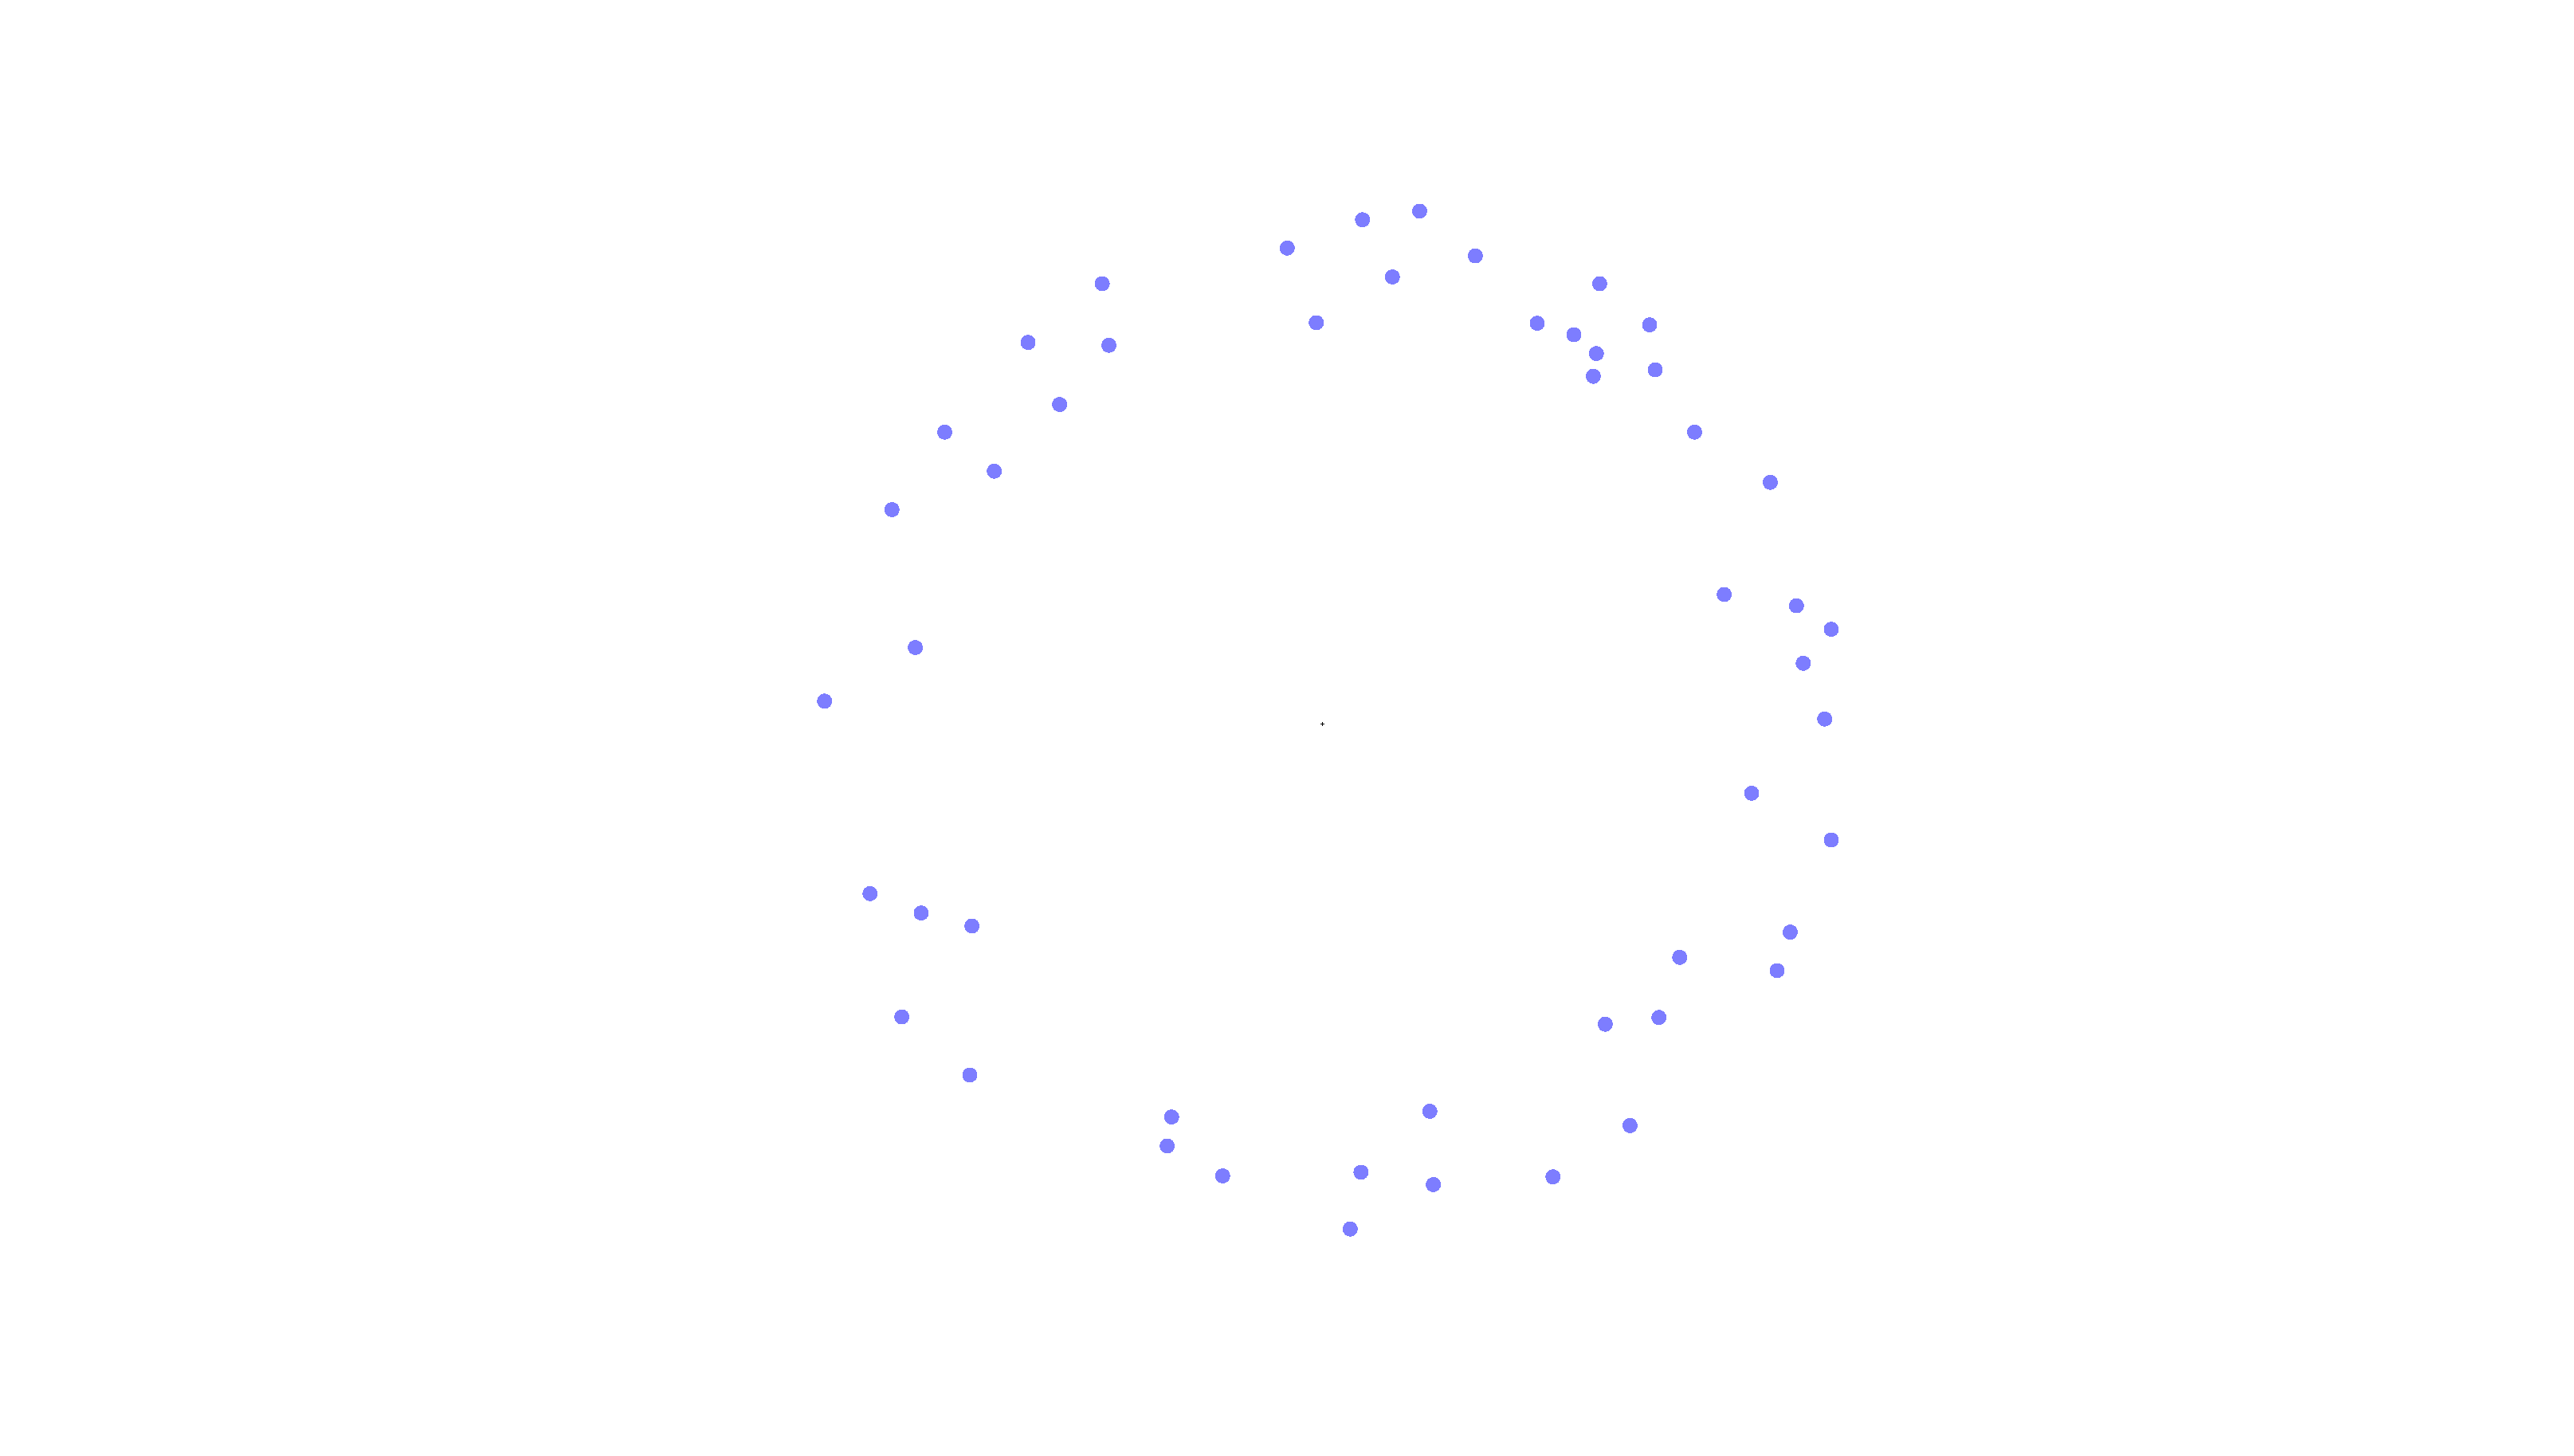
\includegraphics[width=\linewidth]{gfx/statistical_circle.pdf}
    \caption{Campionamento da una corona circolare}
    \label{fig2:circle}
  \end{center}
\end{figure}

Come si possono esprimere queste osservazioni mediante tecniche algebriche? Se i nostri dati sono collezionati nell'insieme finito $X=\{x_1,\dots,x_n\}\subseteq \R^d$, possiamo considerare
\begin{equation*}
  \widehat{X}_\varepsilon = \bigcup_{x\in X} B_\varepsilon(x)
\end{equation*}
dove $B_\varepsilon(x)$ è la palla di raggio $\varepsilon$ e centro $x$. Allora per qualche opportuno $\varepsilon >0$ l'insieme $\widehat{X}_\varepsilon$ associato alla \cref{fig2:clusters} diventa del tipo raffigurato in \cref{fig2:clusters_fat}.

\begin{figure}[h]
  \begin{center}
    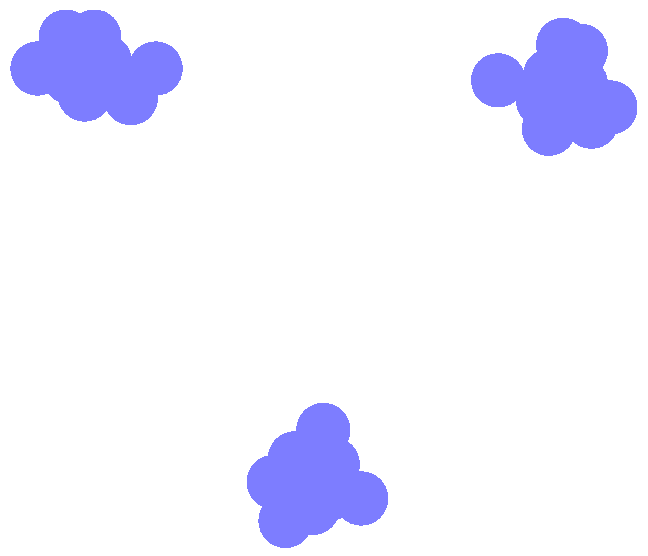
\includegraphics[width=.4\linewidth]{gfx/three_clusters_fat.pdf}
    \caption{$\widehat{X}_\varepsilon$}
    \label{fig2:clusters_fat}
  \end{center}
\end{figure}

Analogamente al variare di $\varepsilon$ vediamo gli spazi mostrati in \cref{fig2:circlecomparison}.

\begin{figure}[h]
  \begin{center}
    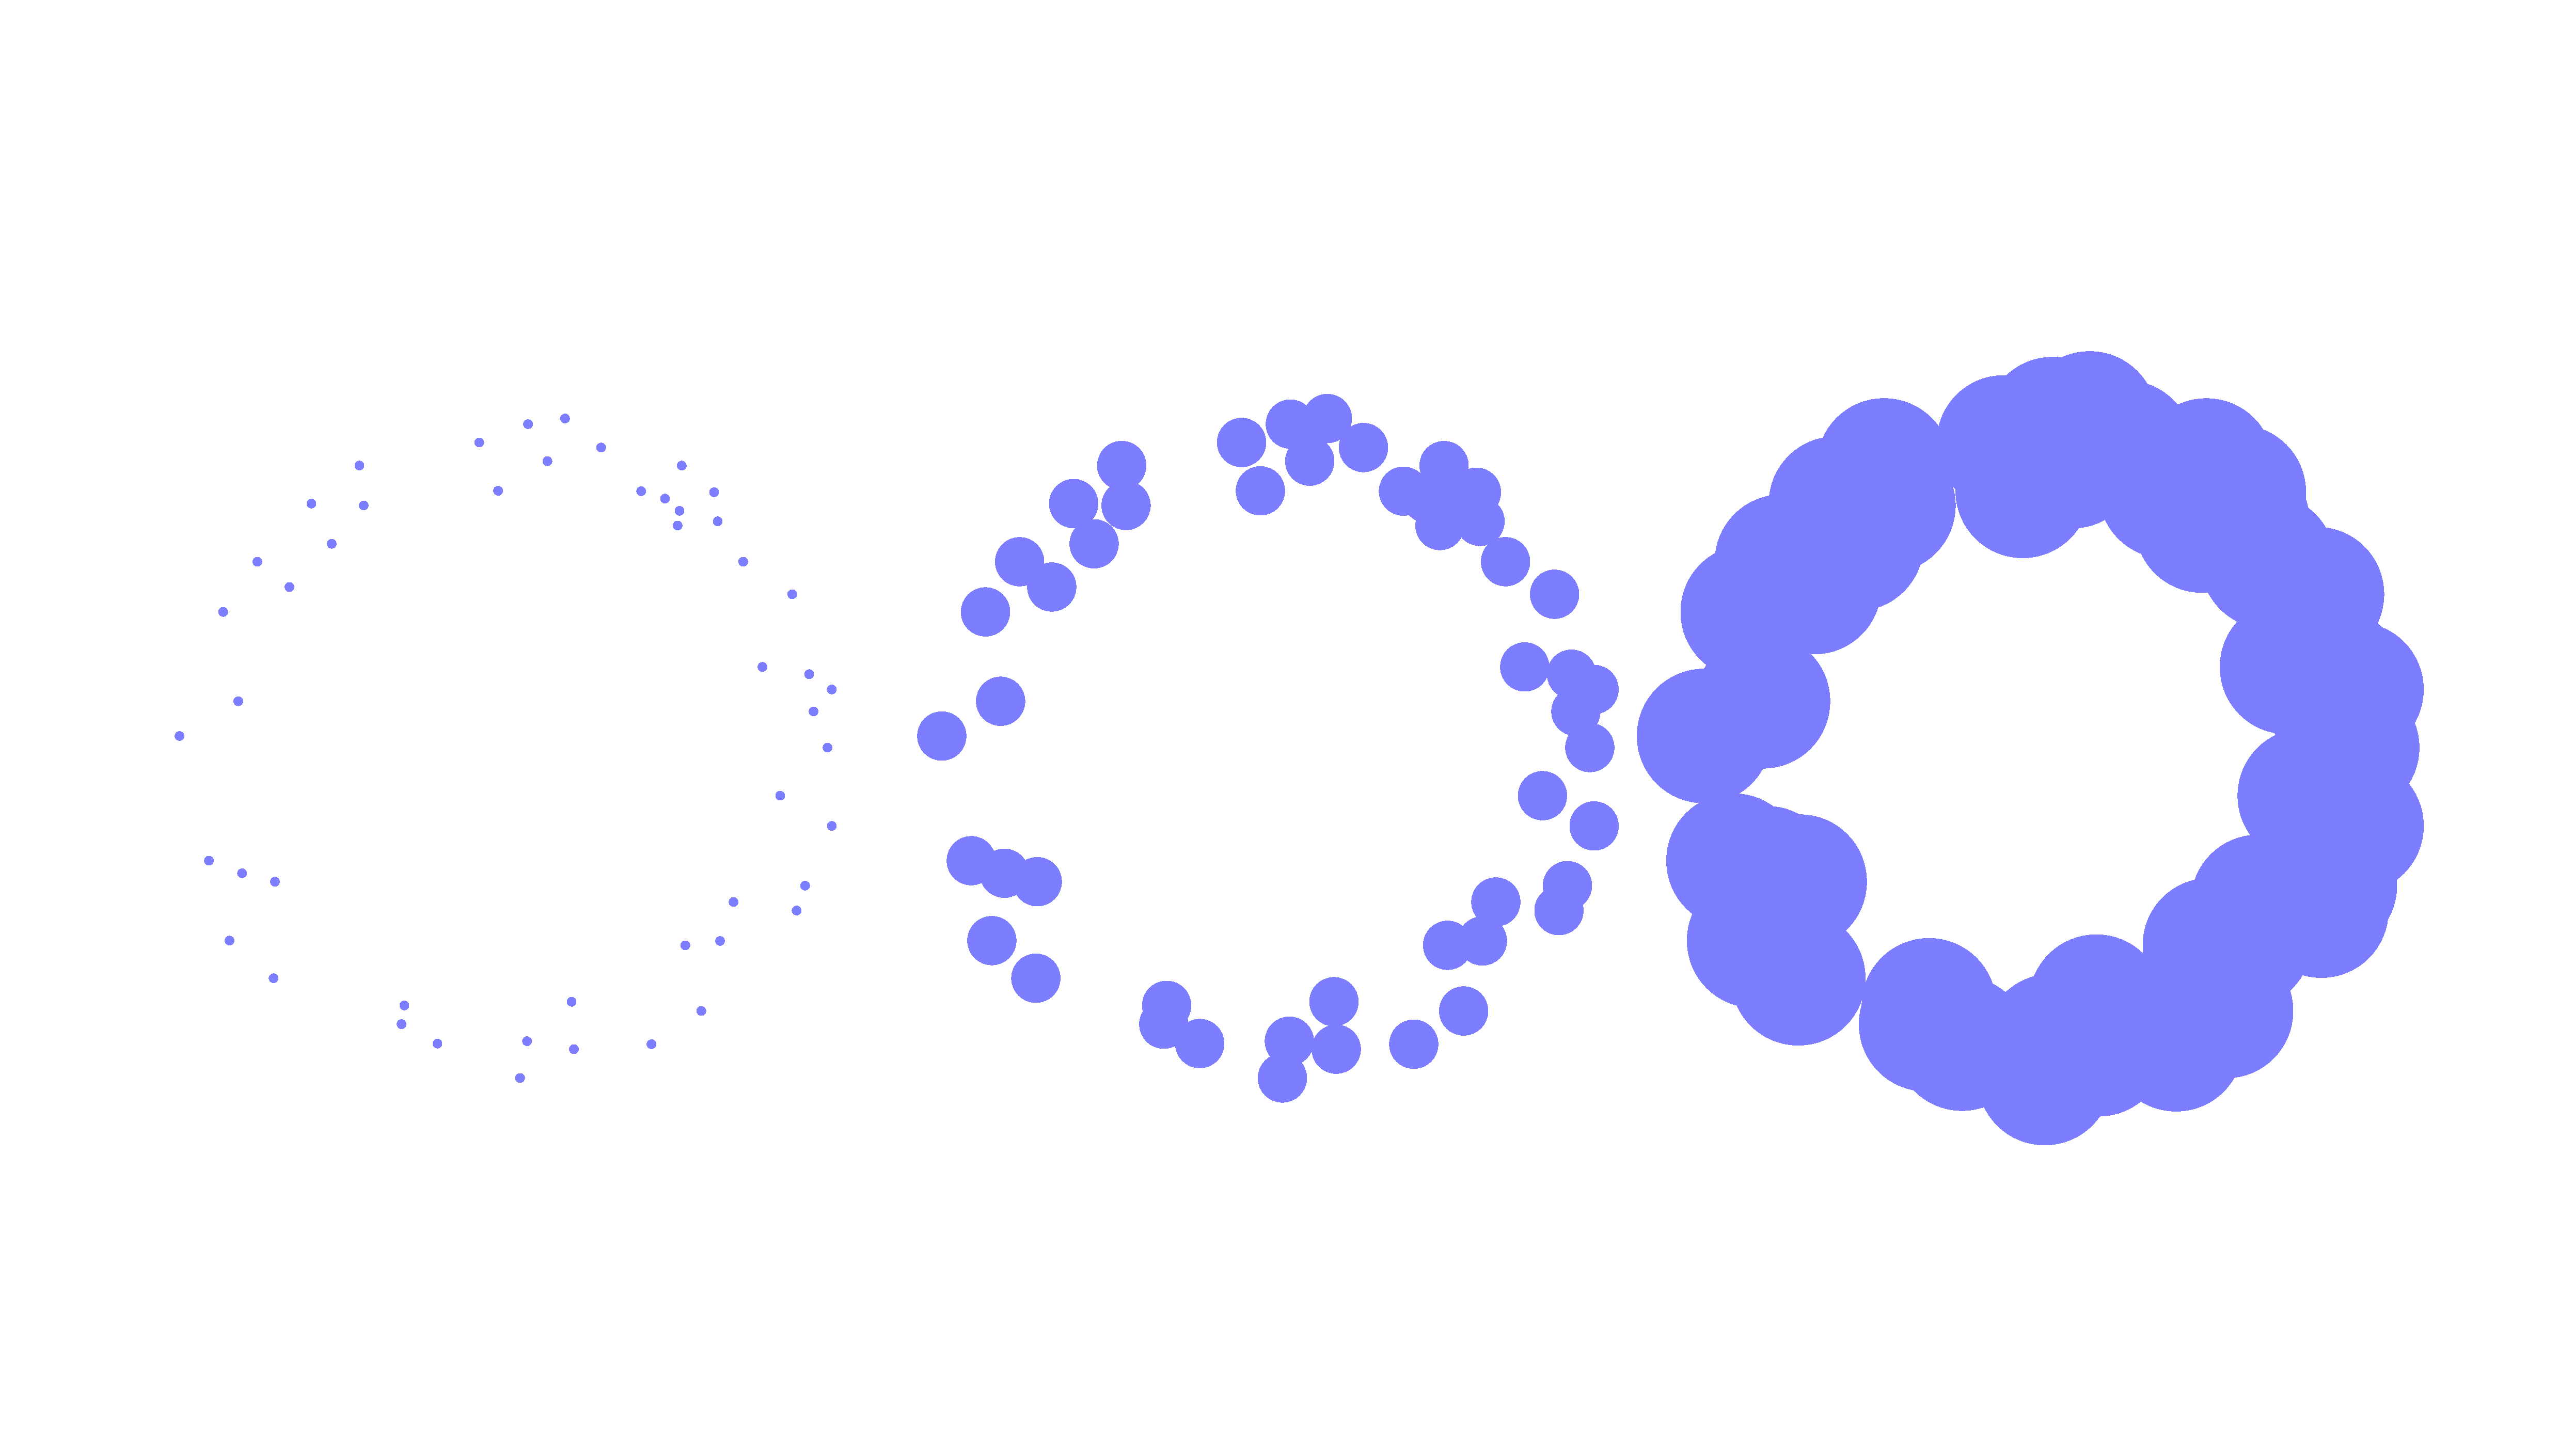
\includegraphics[width=.9\linewidth]{gfx/statistical_circle_comparison.pdf}
    \caption{$\widehat{Y}_\varepsilon$ al variare di $\varepsilon$}
    \label{fig2:circlecomparison}
  \end{center}
\end{figure}

A questo punto abbiamo a che fare con spazi più o meno noti e, per opportune scelte di $\varepsilon$, si possono calcolare i gruppi di omologia $H_0(\widehat{X}_\varepsilon)$ e $H_1(\widehat{Y}_\varepsilon)$ che racchiudono rispettivamente l'informazione sul numero di cluster in \cref{fig2:clusters} e di loop in \cref{fig2:circle}.

Tuttavia in entrambi questi casi c'è bisogno di selezionare un parametro di scala $\varepsilon$ per cui $\widehat{X}_\varepsilon$ contenga esattamente le informazioni che vogliamo trovare, e questa scelta non sempre è evidente. Ad esempio potrebbe succedere che i dati sono in dimensione talmente alta che non è possibile visualizzarli, oppure proprietà che sono evidenti ad una certa scala scompaiono al variare di $\varepsilon$, mentre ne compaiono di nuove. Quindi siamo alla ricerca di metodi che consentano non solo di dedurre informazioni sulla forma dei dati senza doversi preoccupare della selezione di una scala, ma che riescano anche a mettere in relazione le variazioni di queste proprietà al variare della scala di riferimento. L'insieme delle tecniche che consentono di fare questo e molto altro vanno sotto il nome di Topological Data Analysis (TDA).

Lo sviluppo della TDA è stato iniziato da Carlsson et al. nel 2009 in \cite{Carlsson2009}, con l'obiettivo di riuscire a ricavare a partire da un insieme di dati informazioni \emph{qualitative}, \emph{indipendenti dalla scelta di coordinate} e prediligendo una visione d'insieme. Vi sono stati molti progressi sia nella teoria sia nell'applicazione, ad esempio nello sviluppo della teoria della persistenza multidimensionale \cite{Cerri2013,Carlsson2009a,Adcock2012,Carlsson2009b}, della fondazione categorica della persistenza
\cite{Curry}, dell'utilizzo della persistenza nell'inferenza statistica \cite{Bubenik2015,Kwitt2015}, e la ricerca è tuttora in corso.
Alcuni risultati conseguiti utilizzando la TDA sono la determinazione di nuove variabili che influenzano l'attività neurale \cite{Spreemann2015}, la classificazione di traiettorie in robotica \cite{Pokorny2014}, l'identificazione di nuovi tipi di cancro al seno \cite{Lum2013}.

Lo strumento principale della TDA è la omologia persistente, cioé l'assegnazione ad uno spazio metrico finito di una filtrazione di spazi vettoriali $\{V_r\}_{r\in\R}$ in cui gli spazi vettoriali $V_r$ e le mappe fra essi $V_r\to V_s$ per $r<s$ contengano informazioni sulla \emph{forma} dello spazio in esame.

In particolare, gli spazi vettoriali $V_r$ sono gruppi di omologia (e quindi saranno indicati con $H_q(X_r)$) e il parametro $r$ in genere è preso in $\R^+$ perché identifica una scala di riferimento. Questi gruppi di omologia persistenti vengono visualizzati mediante codici a barre persistenti (\cref{fig:typicalbarcode}), dove ogni linea traccia l'evoluzione di una singola \emph{feature} topologica e la lunghezza ne è la durata.

\begin{figure}[h]
  \begin{center}
    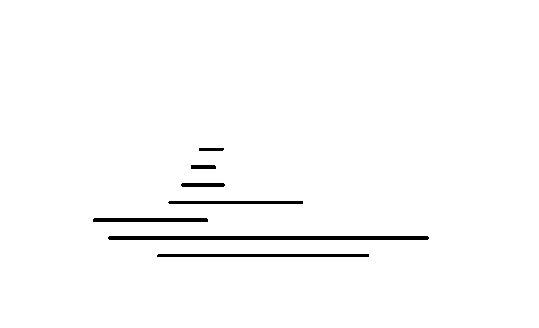
\includegraphics[width=.5\linewidth]{gfx/barcodes_multiple.pdf}
    \caption{Esempio di codice a barre persistente}
    \label{fig:typicalbarcode}
  \end{center}
\end{figure}

La proprietà fondamentale dei gruppi di omologia persistenti è che essi tengono traccia del legame che vi è fra le proprietà topologiche a diverse scale.

\begin{figure}[ht]
  \begin{center}
    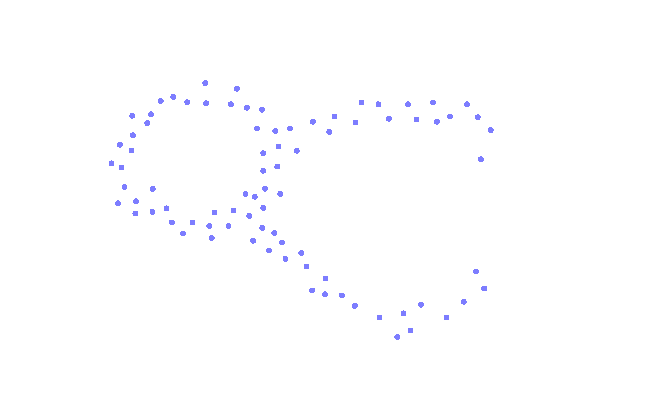
\includegraphics{gfx/double_circle_small.pdf}
    \caption{Un doppio anello}
    \label{fig2:doublecircle}
  \end{center}
\end{figure}

Si consideri ad esempio la nube di punti in \cref{fig2:doublecircle}. Al variare di $r$ compaiono due loop come mostrato in \cref{fig2:doublecirclecomparison}.

\begin{figure}[ht]
  \begin{center}
    \begin{subfigure}[b]{.4\textwidth}
      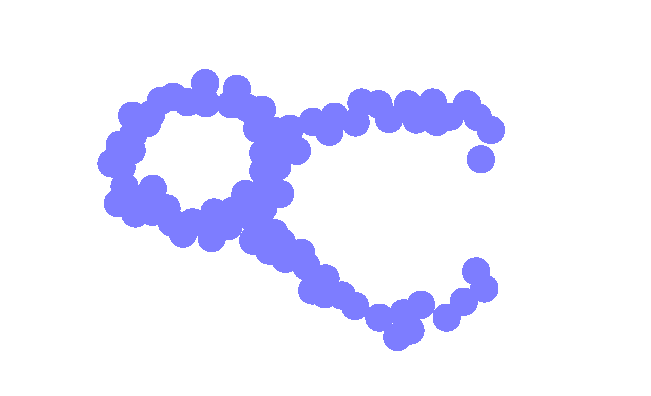
\includegraphics[width=\textwidth]{gfx/double_circle_medium.pdf}
      \caption{$\widehat{X}_{r_1}$}
    \end{subfigure}
    \begin{subfigure}[b]{.4\textwidth}
      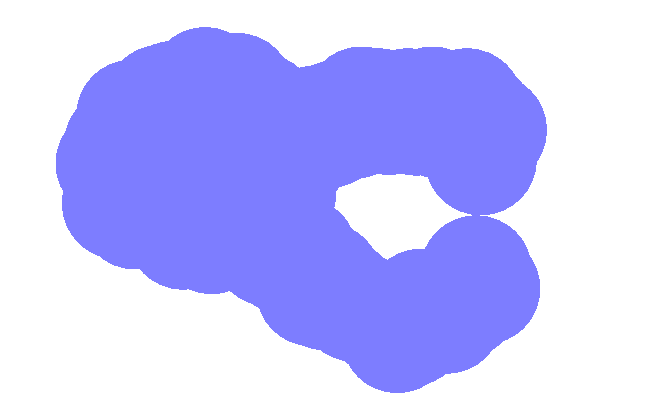
\includegraphics[width=\textwidth]{gfx/double_circle_fat.pdf}
      \caption{$\widehat{X}_{r_2}$}
    \end{subfigure}
    \caption{Variazione delle proprietà di $\widehat{X}_r$}  \label{fig2:doublecirclecomparison}
  \end{center}
\end{figure}

La presenza dei due loop è rappresentata dall'omologia persistente dal fatto che $H_1(\widehat{X}_{r_1})$ e $H_1(\widehat{X}_{r_2})$ hanno entrambi dimensione 1. Tuttavia, l'omologia persistente consente anche di distinguere i due loop. Infatti, poiché $r_1<r_2$ l'omologia persistente viene con una mappa $\psi:H_1(\widehat{X}_{r_1})\to H_1(\widehat{X}_{r_2})$ e il fatto che i due loop sono distinti lo si deduce dal fatto che $\psi=0$.

Questa proprietà dell'omologia persistente, dettà \emph{funtorialità}, è l'elemento essenziale che rende queste tecniche estremamente utili nelle applicazioni.

L'altra proprietà fondamentale dell'omologia persistente è enunciata nel \Cref{thm:persistentdecomposition} che garantisce che ogni gruppo di omologia persistente associato ad uno spazio metrico finito può essere rappresentato con un numero finito (idealmente piccolo) di parametri. Questo fatto consente di visualizzare con pochi parametri un insieme di dati potenzialmente complesso, inoltre lo spazio di questi parametri può essere reso uno spazio metrico completo (come in \cite{Kwitt2015}), aprendo spazio all'utilizzo di tecniche di statistica e machine learning.

Nel \cref{ch:teoria} ci occuperemo di sviluppare l'omologia persistente, richiamando velocemente le nozioni necessarie di topologia algebrica e in particolare l'omologia simpliciale, mentre nel \cref{cap:esempi} mostreremo alcuni esempi su dati sintetici di codici a barre persistenti.
